\chapter{Electric Transport Technology}
\section{Electric railways (UK)}
\begin{itemize}
    \item 1883 - first electric rail system in UK known as the Volks Electric Railway in Brighton
    \item 1890 - London Underground adopted elcetrical power on parts of its network. This quickly advanced to the whole system
    \item 1920s - \SI{660}{\volt} DC rail for overground rail system known as third rail system. Later \SI{750}{\volt} DC
    \item 1956 - \SI{25}{\kilo\volt} single-phase overhead line system adopted on some main lines
    \item Today around 47\% of the network is electrified using DC and AC power systems
\end{itemize}
\section{Types of transit systems}
\begin{figure}[H]
    \centering
    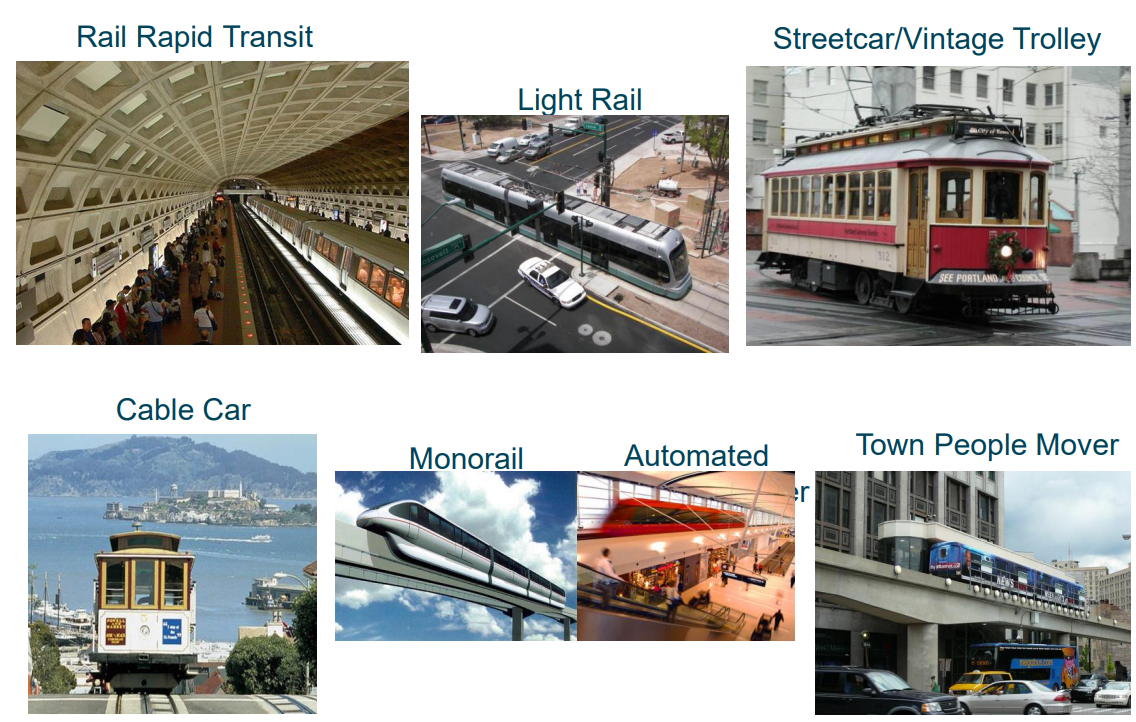
\includegraphics[width = 0.8\textwidth]{img/figure116.png}
    \caption{Types of transit system.}
\end{figure}
\section{Question 1 - Consider two requirements of an ideal traction system}
Requirments:
\begin{itemize}
    \item The starting tractive effort should be high so as to have rapid acceleration
    \item The wear on the track should be minimum
    \item The equipments should be capable of withstanding large temporary loads
    \item Speed control should be easy
    \item Pollution free
    \item Low initial and maintenance cost
    \item The locomotive should be self-contained and able to run on any route
\end{itemize}
\section{Power supply}
\subsection{Incoming supply (AC lines)}
\begin{figure}[H]
    \centering
    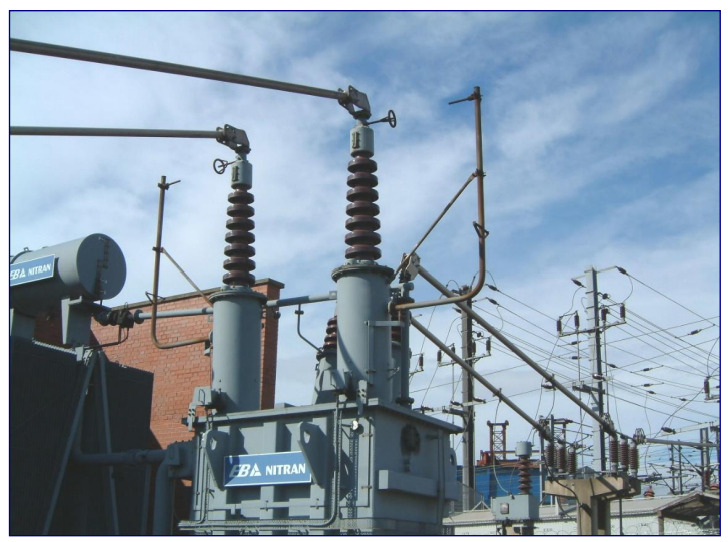
\includegraphics[width = 0.8\textwidth]{img/figure117.png}
    \caption{Network Rail is supplied with \SI{25}{\kilo\volt} (single-phase) by DNOs at Feeder Stations for its classic OLE system.}
\end{figure}
\subsection{Incoming supply (DC lines)}
\begin{figure}[H]
    \centering
    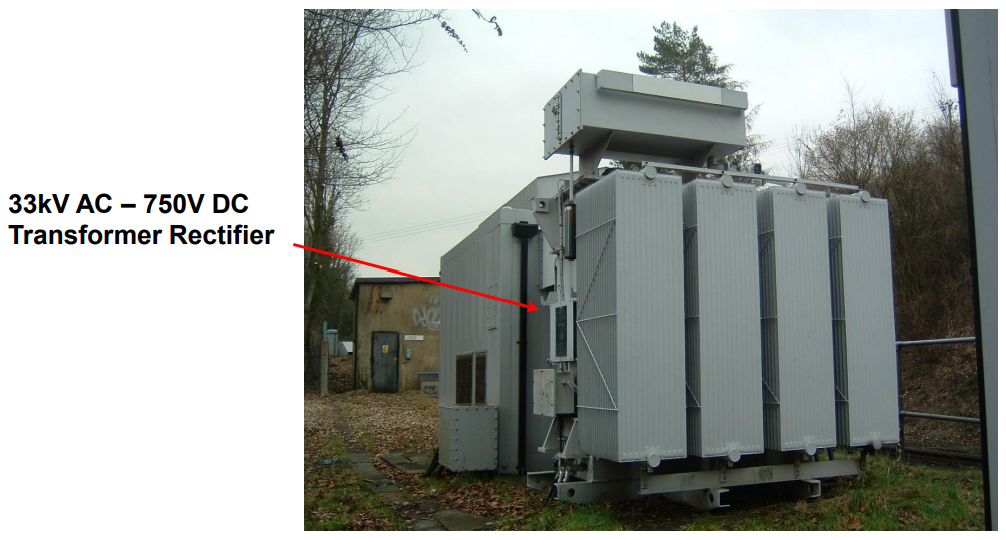
\includegraphics[width = 0.8\textwidth]{img/figure118.png}
    \caption{Network Rail is supplied with \SI{11}{\kilo\volt}, \SI{22}{\kilo\volt} or \SI{33}{\kilo\volt} (three-phase) by DNOs. The supply is then passed through a step-down transformer and rectifiers to provide \SI{750}{\volt} DC for conductor rail feeding.}
\end{figure}
\subsection{Lineside substations}
\begin{figure}[H]
    \centering
    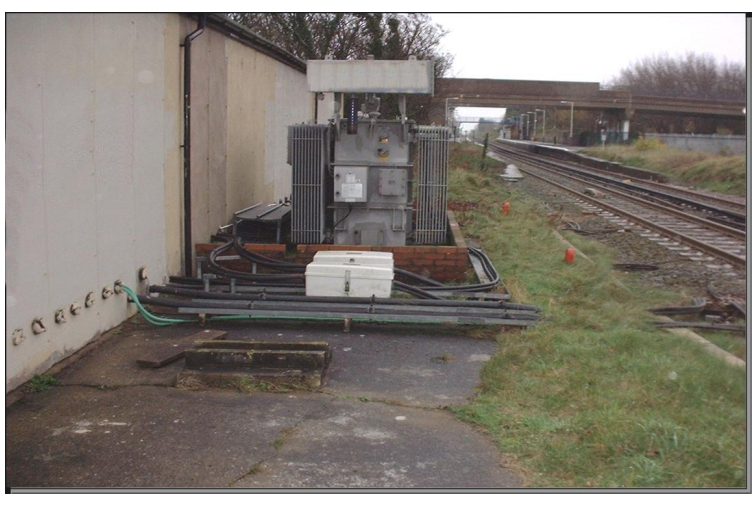
\includegraphics[width = 0.8\textwidth]{img/figure119.png}
    \caption{Lineside substation.}
\end{figure}
Conductor rail systems use lineside substations where the high voltage is stepped down and recitified for track feeding. The voltage at the conductor rail is suitable for traction purposes i.e. no further reduction occurs on board the train.
\subsection{Circuit breakers}
\begin{figure}[H]
    \centering
    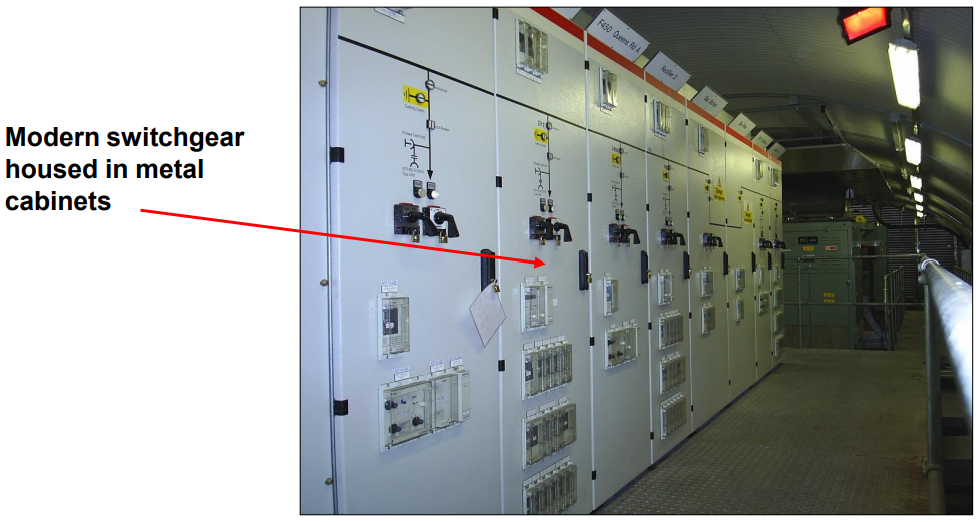
\includegraphics[width = 0.8\textwidth]{img/figure120.png}
    \caption{Circuit breakers.}
\end{figure}
High speed circuit breakers are used for traction circuit protection purposes. They are remotely controlled and are opened to provide electrical isolations for planned work or for emergency switch off.
\subsubsection{Deciding the type of circuit breaker}
\begin{itemize}
    \item Continuous amps
    \item Long time delay
    \item Short time pick-up
    \item Short time delay
    \item Ground fault pick-up
\end{itemize}
\subsection{Electrical Control Room (ECR)}
\begin{figure}[H]
    \centering
    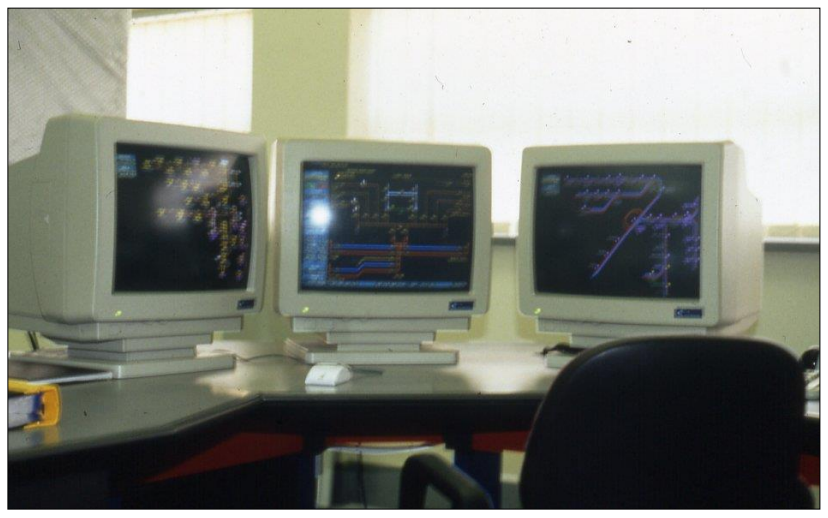
\includegraphics[width = 0.8\textwidth]{img/figure121.png}
    \caption{Electrical Control Room (ECR).}
\end{figure}
Electrical Control Rooms (13 across the network) are staffed continually by Electrical Control Operators (ECOs). All equipment is monitored and controlled remotely from the ECRs.
\section{DC power systems}
\subsection{Types of conductor rail}
\begin{figure}[H]
    \centering
    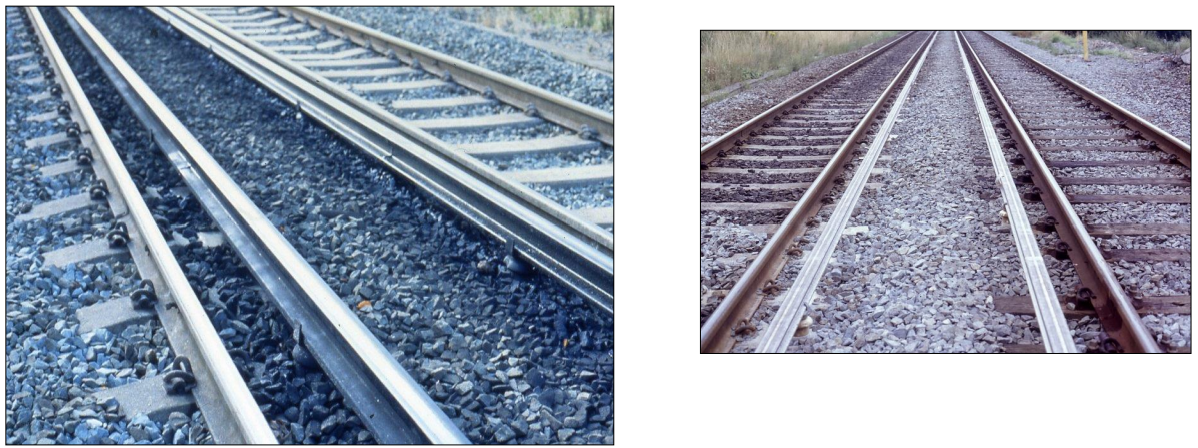
\includegraphics[width = 0.8\textwidth]{img/figure122.png}
    \caption{Conductor rails (DC).}
\end{figure}
Conductor rails are made from steel or aluminium alloy with a stainless steel top surface (composite) and are mounted on porcelain or plastic insulators secured to the sleeper ends.
\begin{figure}[H]
    \centering
    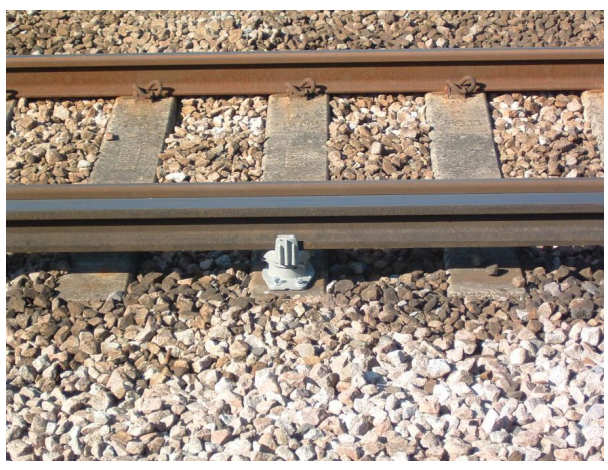
\includegraphics[width = 0.8\textwidth]{img/figure123.png}
    \caption{Insulators (DC).}
\end{figure}
The primary purpose of insulators is to prevent the conductor rail from discharging to earth. Insulators and their associated components also provide the mechanical means of adjusting the height at which the conductor rail is set in relation to the running rails.
\subsection{Conductor rail ramp ends}
\begin{figure}[H]
    \centering
    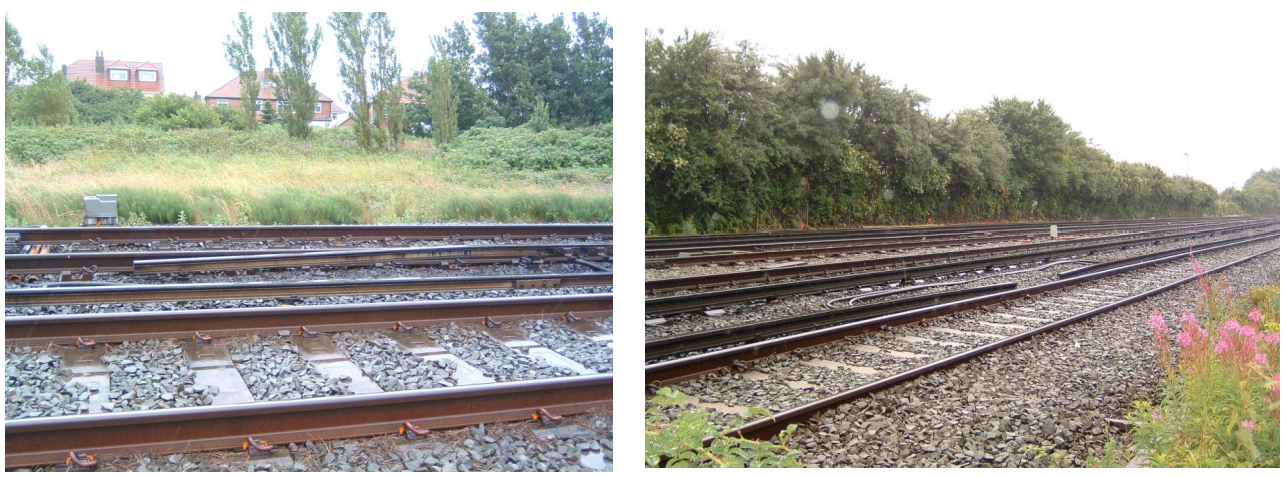
\includegraphics[width = 0.8\textwidth]{img/figure124.png}
    \caption{Conductor rail ramp ends.}
\end{figure}
The conductor rail is `ramped' at section gaps and expansion gaps in order to facilitate the smooth passage of the collector shoes. The length (and therefore the gradient) of the ramps is determined by permitted line speed.
\subsection{Current collection}
\begin{figure}[H]
    \centering
    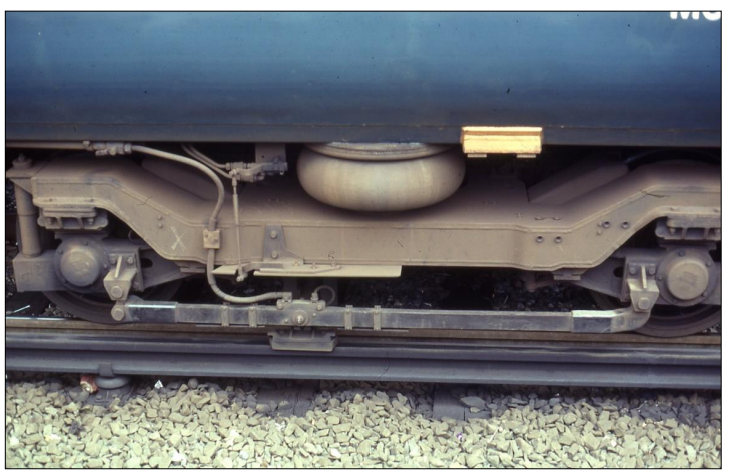
\includegraphics[width = 0.8\textwidth]{img/figure125.png}
    \caption{Current collection.}
\end{figure}
Traction current is collected by the train's collector shoes and passes through the motors and auxillary circuits before returning to the substation via the axles, wheels and one or both of the running rails. 
\subsection{Conductor rail positioning}
\begin{figure}[H]
    \centering
    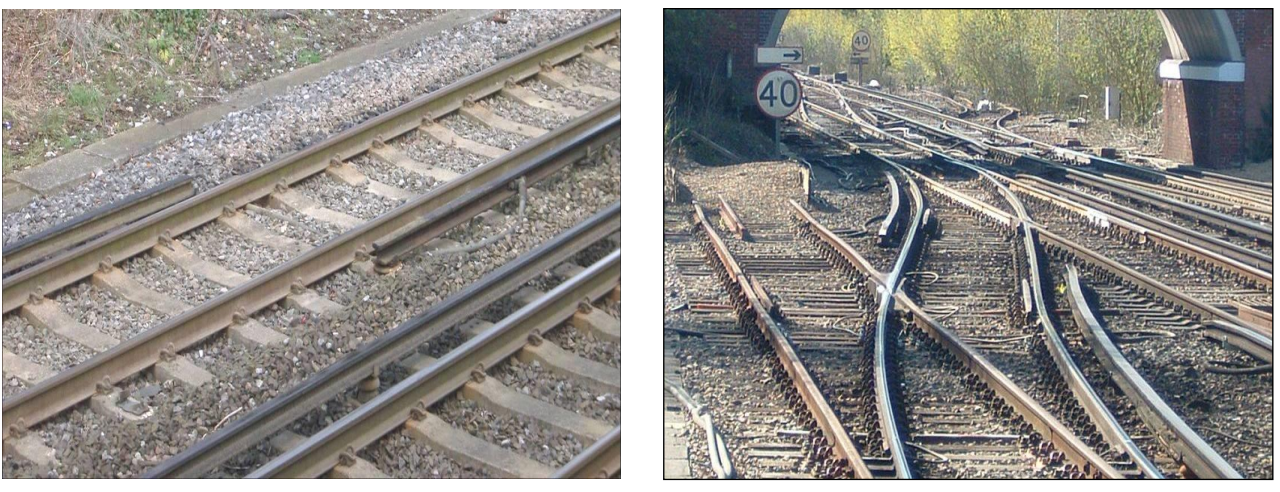
\includegraphics[width = 0.8\textwidth]{img/figure126.png}
    \caption{Conductor rail positioning.}
\end{figure}
Conductor rail can be bolted to the sleeper ends on either side of the track. Where necessary, electrical continuity is achieved by cable bonds. 
\subsection{Traction current return}
\begin{figure}[H]
    \centering
    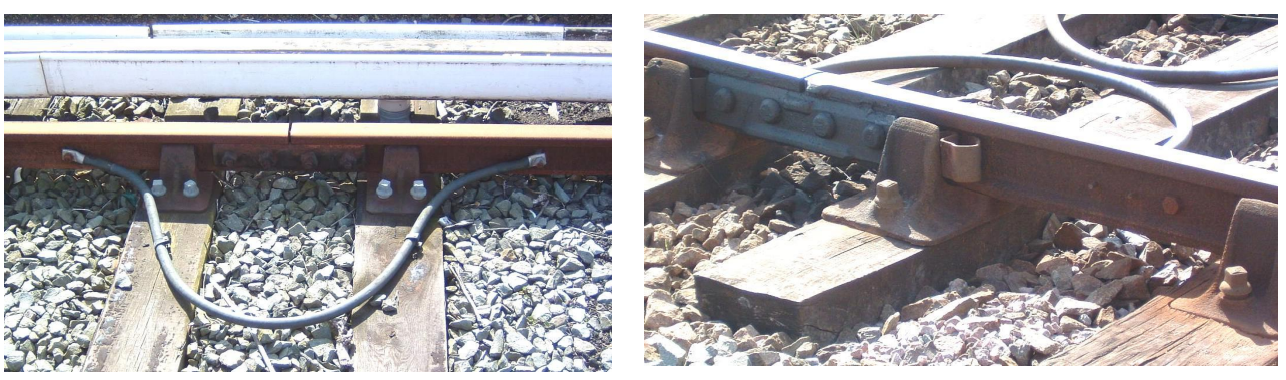
\includegraphics[width = 0.8\textwidth]{img/figure127.png}
    \caption{Traction current return.}
\end{figure}
Fish-plated rail joints in a rail used for traction current return purposes must be bridged by bonds to assure the availability of a continuous low resistance path. Greater use of continuously welded rail has reduced the need for this type of bond, resulting in reduced maintenance costs and aesthetic benefits. 
\subsection{Feeding the conductor rail}
\begin{figure}[H]
    \centering
    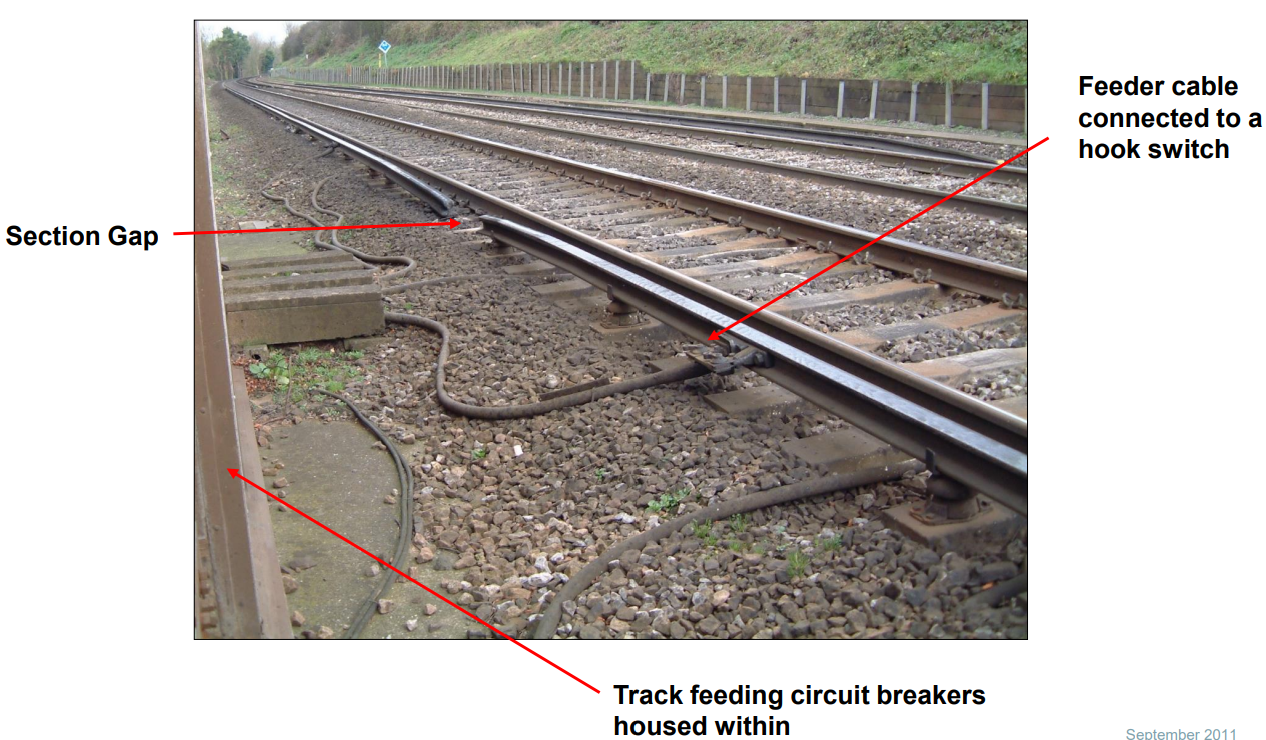
\includegraphics[width = 0.8\textwidth]{img/figure128.png}
    \caption{Feeding the conductor rail.}
\end{figure}
\subsection{Manually operated switches}
\begin{figure}[H]
    \centering
    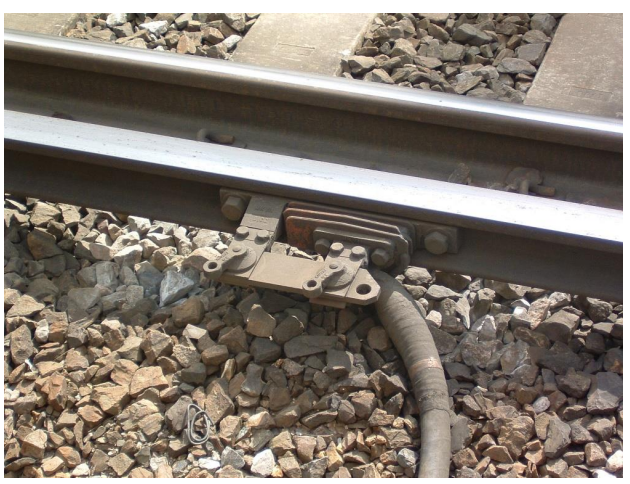
\includegraphics[width = 0.8\textwidth]{img/figure129.png}
    \caption{Manually operated switch.}
\end{figure}
Switches are provided to facilitate the splitting of electrical sections into subsections (including electrified sidings) for strategic isolation purposes. They are manually operated using a wooden pole with a hook on the end - hence the term `hook switch.'
\section{Question 2 - Consider two earth return paths that may be used with third rail systems}
Through one of the track rails e.g. overland. By using a fourth rail e.g. London Underground.
\section{AC Power Systems}
\subsection{AC overhead electrified lines}
\begin{figure}[H]
    \centering
    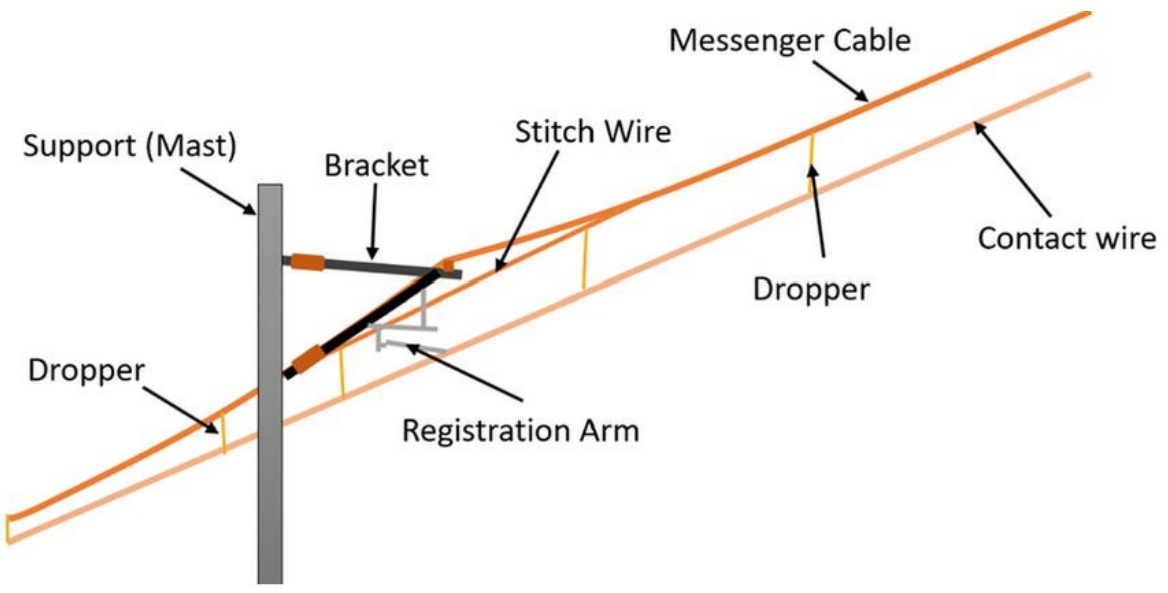
\includegraphics[width = 0.8\textwidth]{img/figure130.png}
    \caption{Component of AC overhead electrified lines.}
\end{figure}
\subsection{Feeding OLE}
\begin{figure}[H]
    \centering
    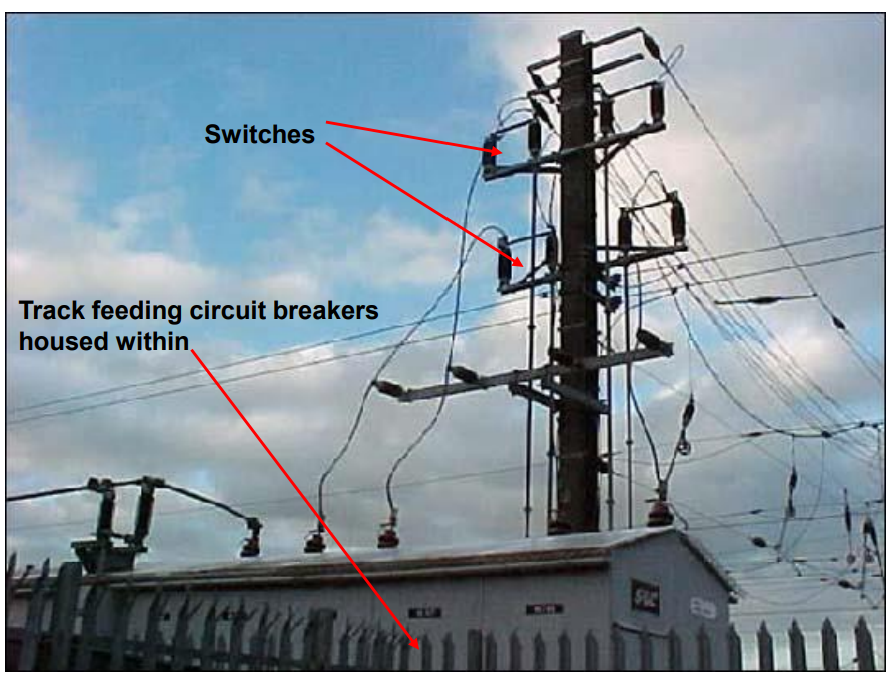
\includegraphics[width = 0.8\textwidth]{img/figure131.png}
    \caption{Feeding OLE.}
\end{figure}
\subsection{System of supply}
\SI{25}{\kilo\volt} AC single phase. For traction substation (TSS) the incoming EHV supply is 220/132/\SI{110}{\kilo\volt}. Through protective equipment it can be transformed by using the traction transformer to \SI{25}{\kilo\volt} AC single phases. Spacing between TSS is \SI{30}{\kilo\meter} to \SI{40}{\kilo\meter} depending upon the traffic (load). To avoid load on one phase and balancing the incoming supply grid, the section TSS is divided into sub-sector through switching posts. 
\begin{enumerate}
    \item S.P. - sectioning and paralleling post
    \item S.S.P. - sub-sectioning and parelleling post
\end{enumerate}
\subsection{High speed rail (HSR)}
A rail line and service designed for high-speed operations - 250-\SI{400}{\kilo\meter\per\hour}. Straight line tracks and designated corridors.
\begin{figure}[H]
    \centering
    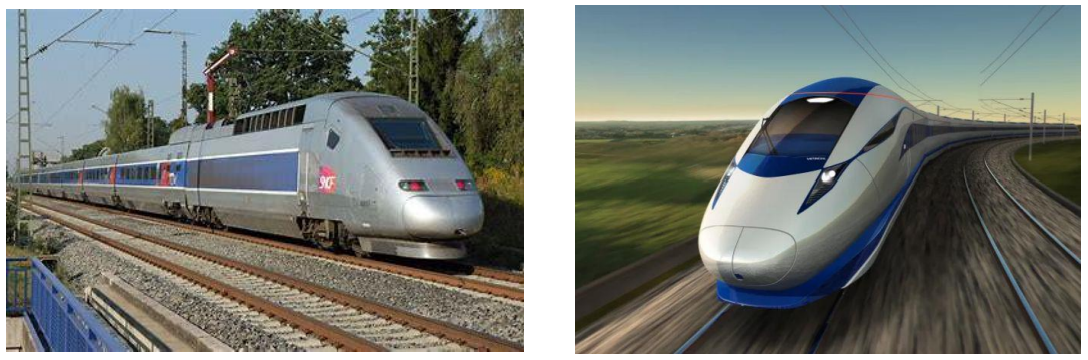
\includegraphics[width = 0.8\textwidth]{img/figure132.png}
    \caption{High speed rail.}
\end{figure}
\subsection{On-board `substations'}
\begin{figure}[H]
    \centering
    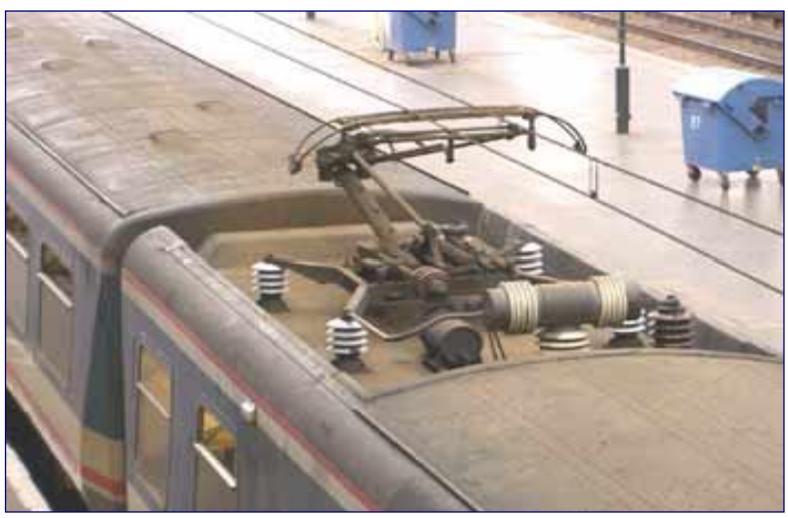
\includegraphics[width = 0.8\textwidth]{img/figure133.png}
    \caption{High speed rail.}
\end{figure}
\SI{25}{\kilo\volt} AC is used for power transmission purposes on OLE systems. Traction motors driving the wheels of trains require a much lower operating voltage, achieved using on-board step-down transformers. 
\subsection{Conventional AC electric locomotive}
\begin{figure}[H]
    \centering
    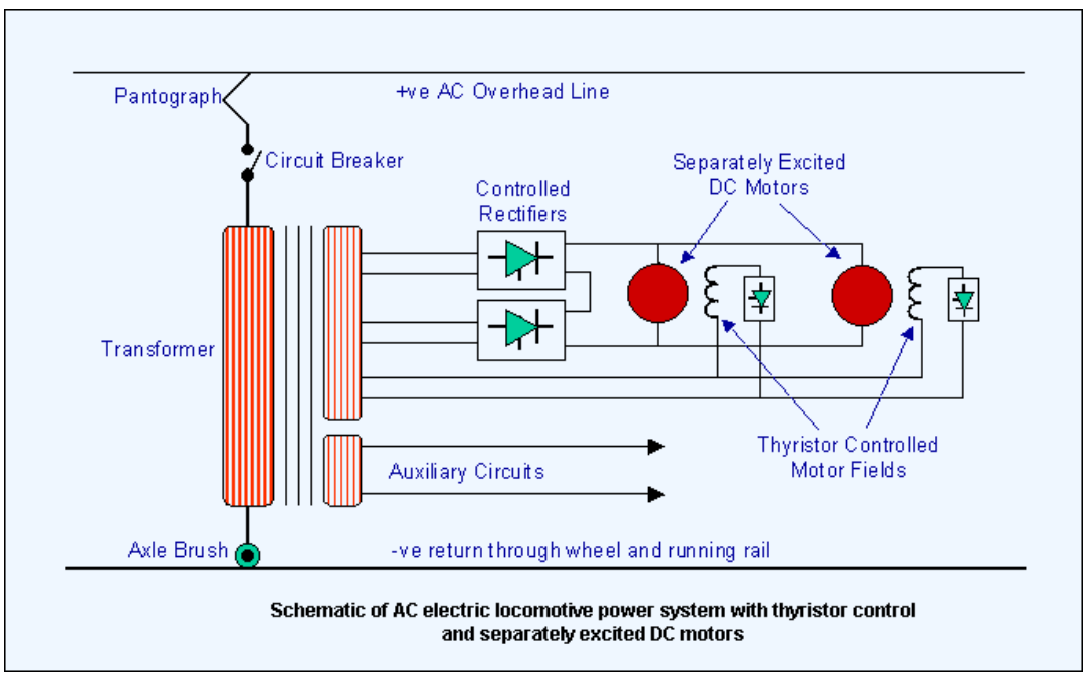
\includegraphics[width = 0.8\textwidth]{img/figure134.png}
    \caption{Schematic of AC electric locomotive power system with thyristor control and separately excited DC motors.}
\end{figure}
\subsection{Modern AC electric locomotive}
\begin{figure}[H]
    \centering
    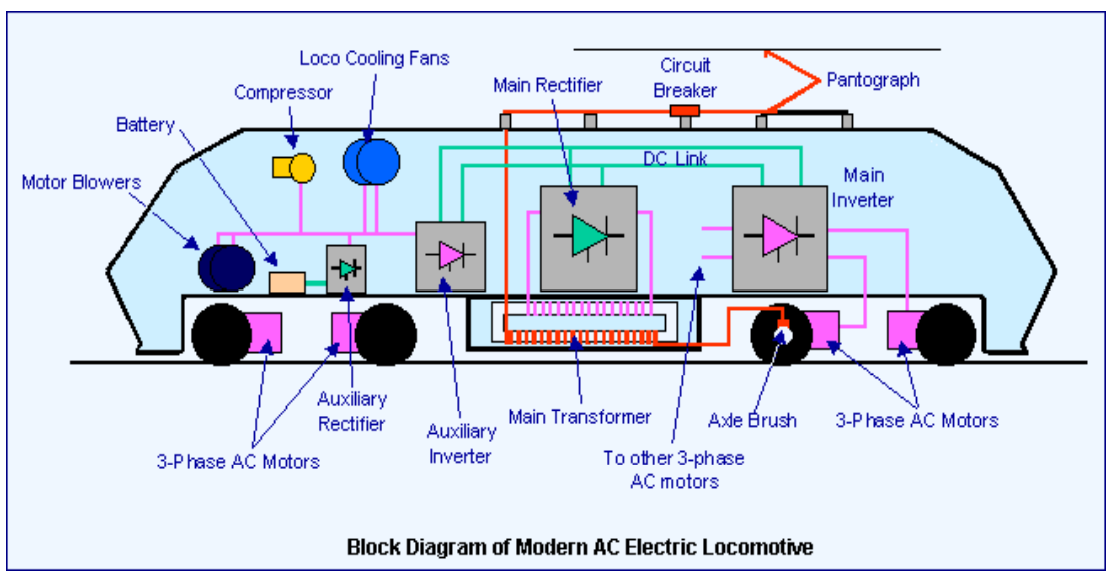
\includegraphics[width = 0.8\textwidth]{img/figure135.png}
    \caption{Block diagram of modern AC electric locomotive.}
\end{figure}
\subsection{Overhead line equipment}
\begin{figure}[H]
    \centering
    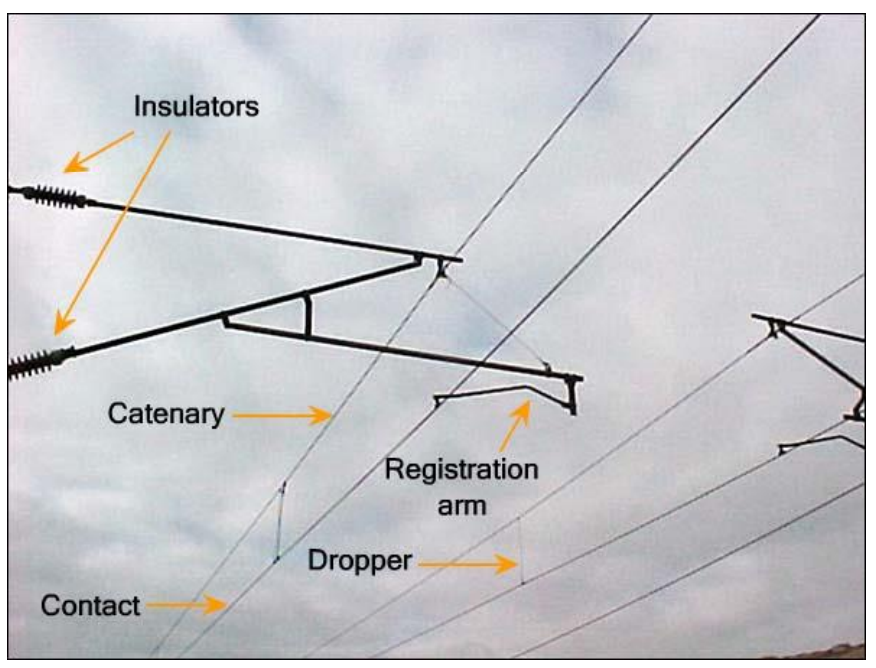
\includegraphics[width = 0.8\textwidth]{img/figure136.png}
    \caption{Overhead line equipment.}
\end{figure}
\subsection{Neutral sections}
\begin{figure}[H]
    \centering
    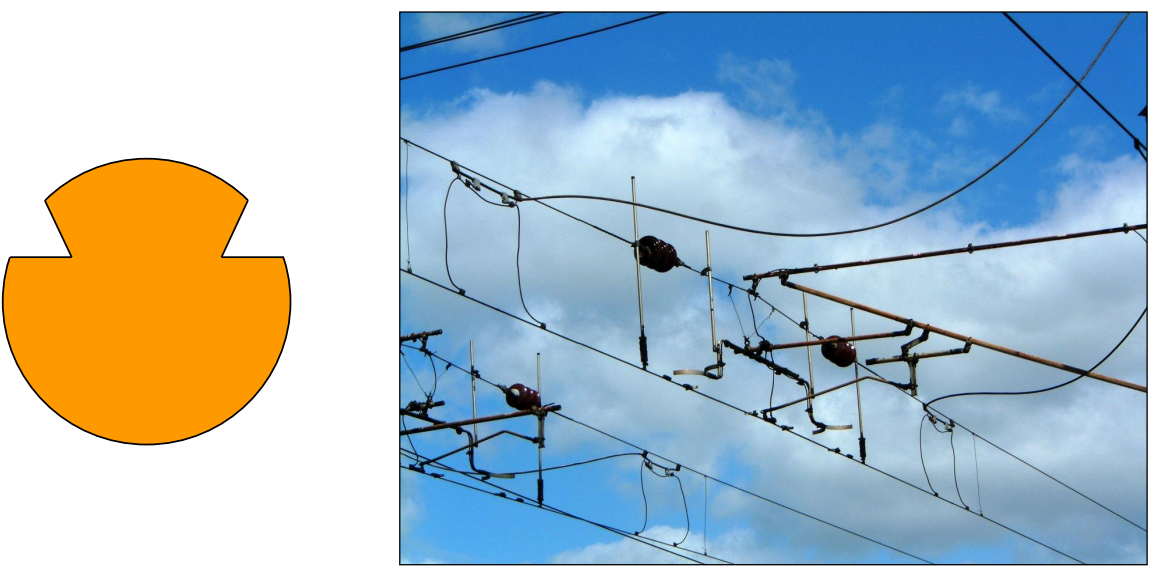
\includegraphics[width = 0.8\textwidth]{img/figure137.png}
    \caption{Various designs of neutral section exist, this example being BICC. Note the cross-section of the conductor wire.}
\end{figure}
\subsection{Insulators}
\begin{figure}[H]
    \centering
    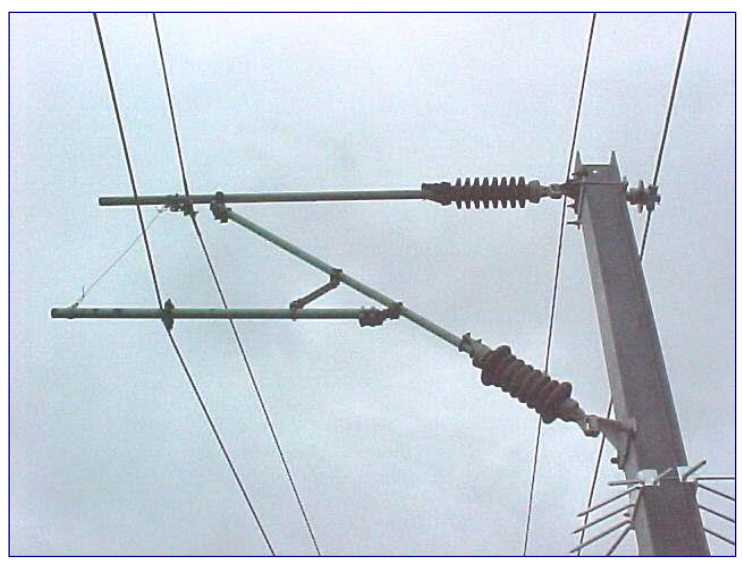
\includegraphics[width = 0.8\textwidth]{img/figure138.png}
    \caption{Insulator.}
\end{figure}
Insulators are used to prevent the live overhead line equipment discharging to earth through the main steelwork. 
\subsection{Section insulators}
\begin{figure}[H]
    \centering
    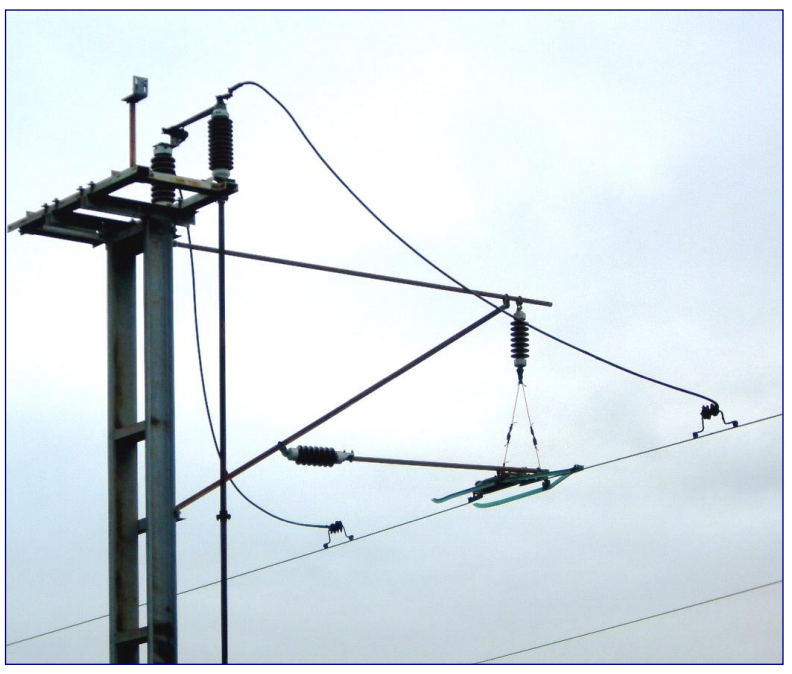
\includegraphics[width = 0.8\textwidth]{img/figure139.png}
    \caption{Section insulator.}
\end{figure}
\subsection{Section insulators}
\begin{figure}[H]
    \centering
    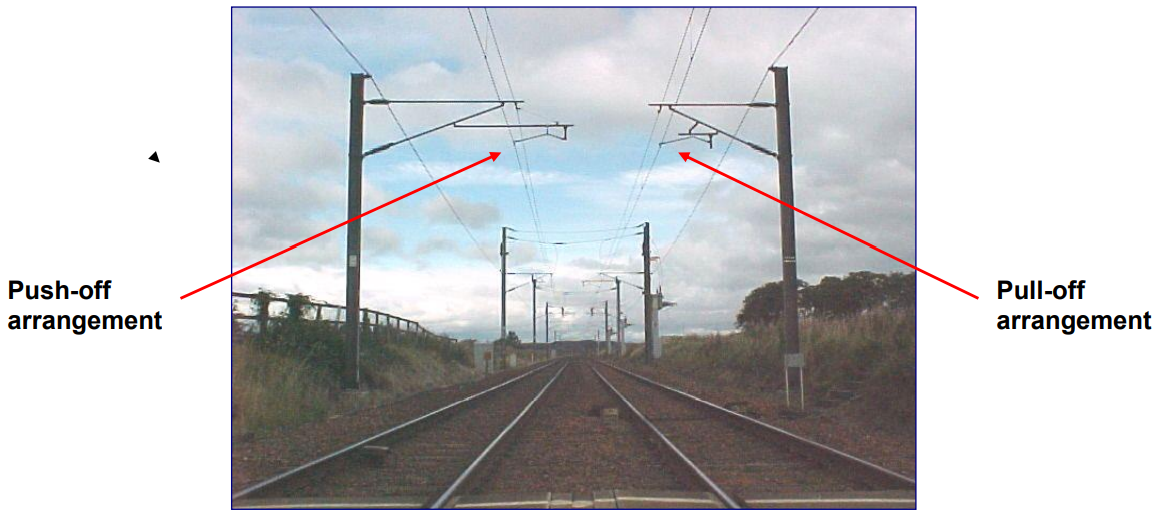
\includegraphics[width = 0.8\textwidth]{img/figure140.png}
    \caption{Stagger.}
\end{figure}
The contact wire is `staggered' to prevent concentrated wear on the train's pantograph (current collecting equipment) i.e. it zigzags along the track.
\begin{figure}[H]
    \centering
    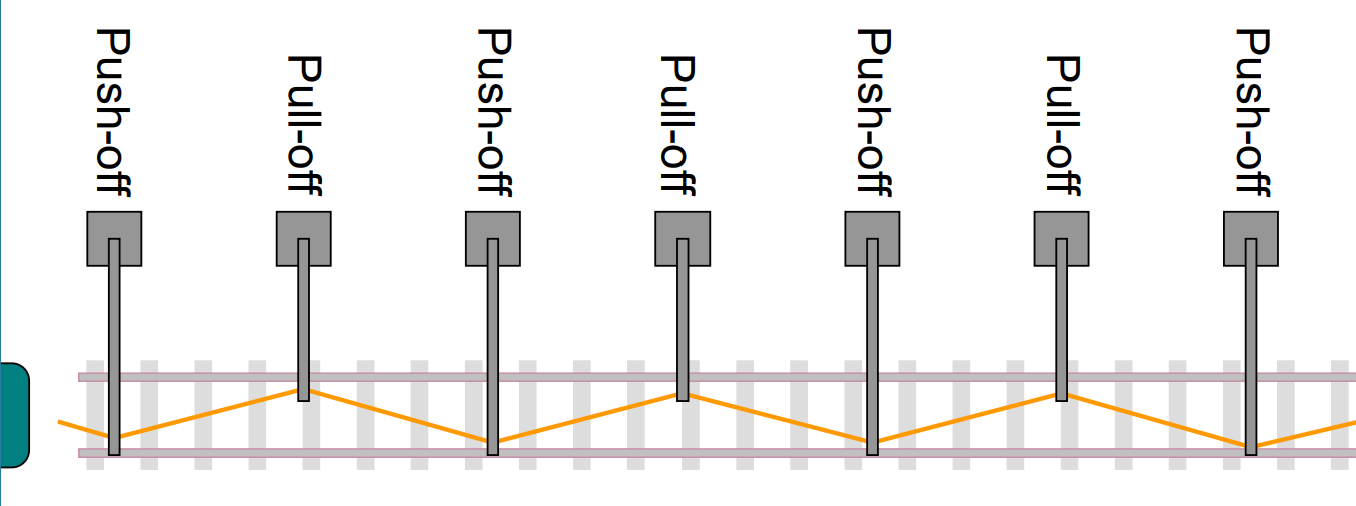
\includegraphics[width = 0.8\textwidth]{img/figure141.png}
    \caption{Stagger overhead view.}
\end{figure}
\subsection{Headspan structures}
\begin{figure}[H]
    \centering
    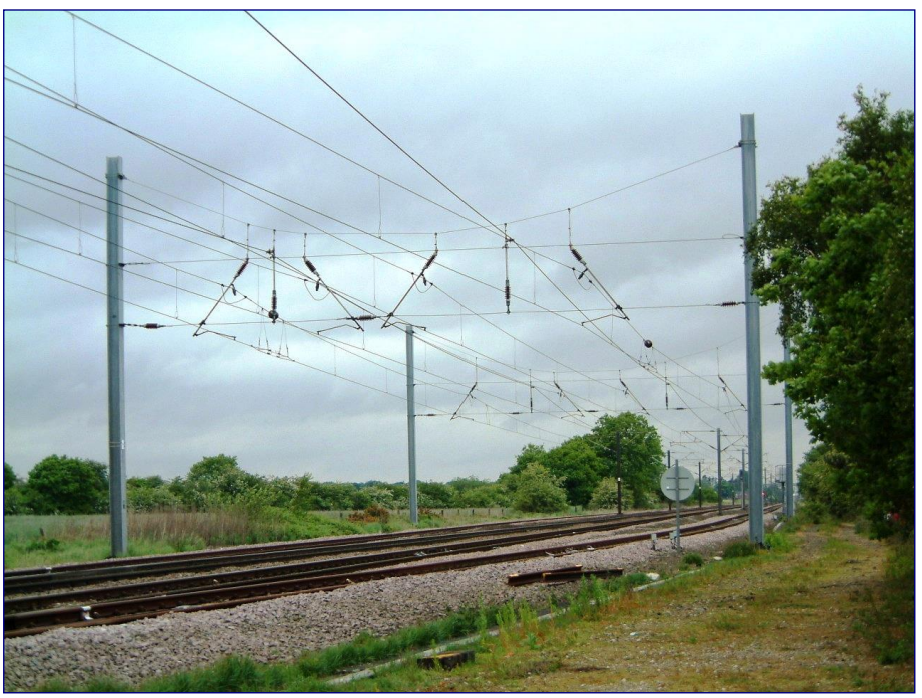
\includegraphics[width = 0.8\textwidth]{img/figure142.png}
    \caption{Headspan structure.}
\end{figure}
\begin{figure}[H]
    \centering
    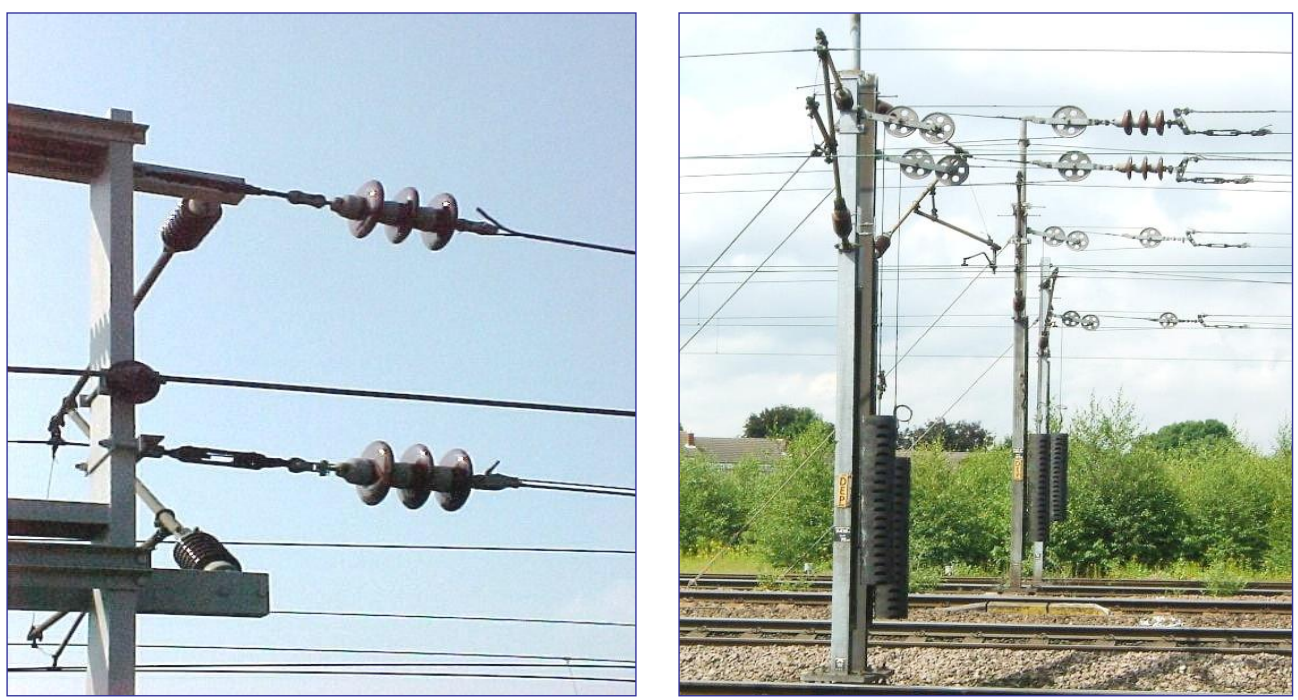
\includegraphics[width = 0.8\textwidth]{img/figure143.png}
    \caption{Headspan structure (fixed and auto-tensioned).}
\end{figure}
\begin{figure}[H]
    \centering
    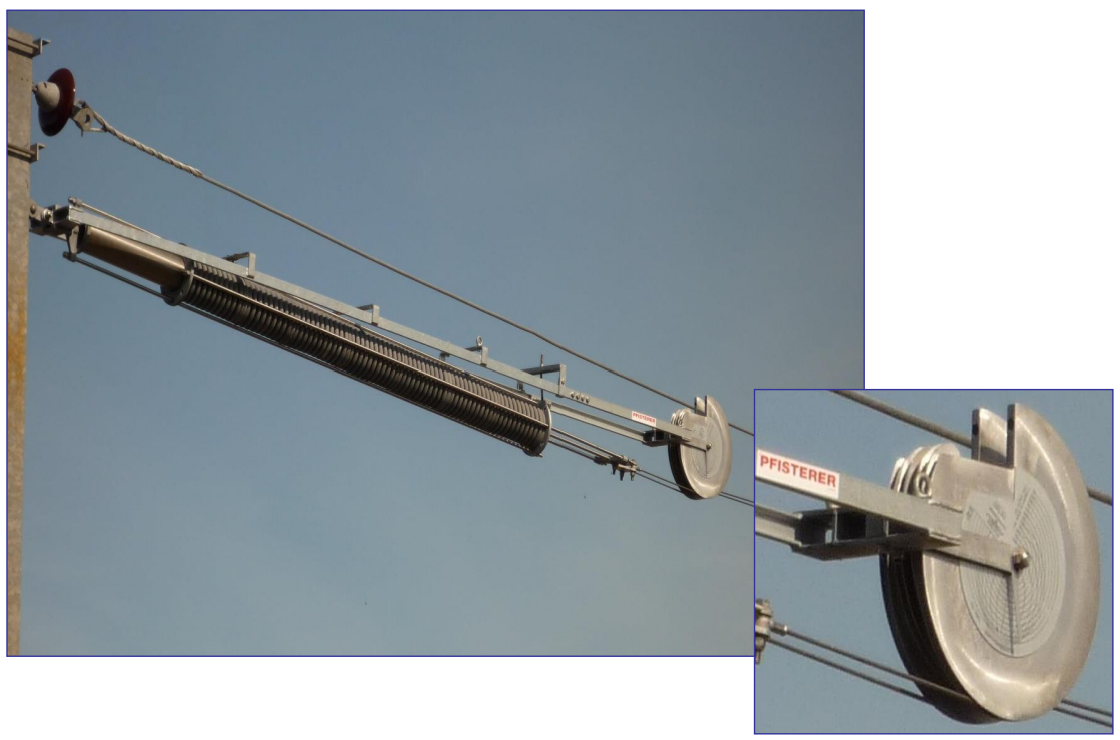
\includegraphics[width = 0.8\textwidth]{img/figure144.png}
    \caption{Headspan structure (spring-tensioned).}
\end{figure}
\subsection{Isolators / switches}
\begin{figure}[H]
    \centering
    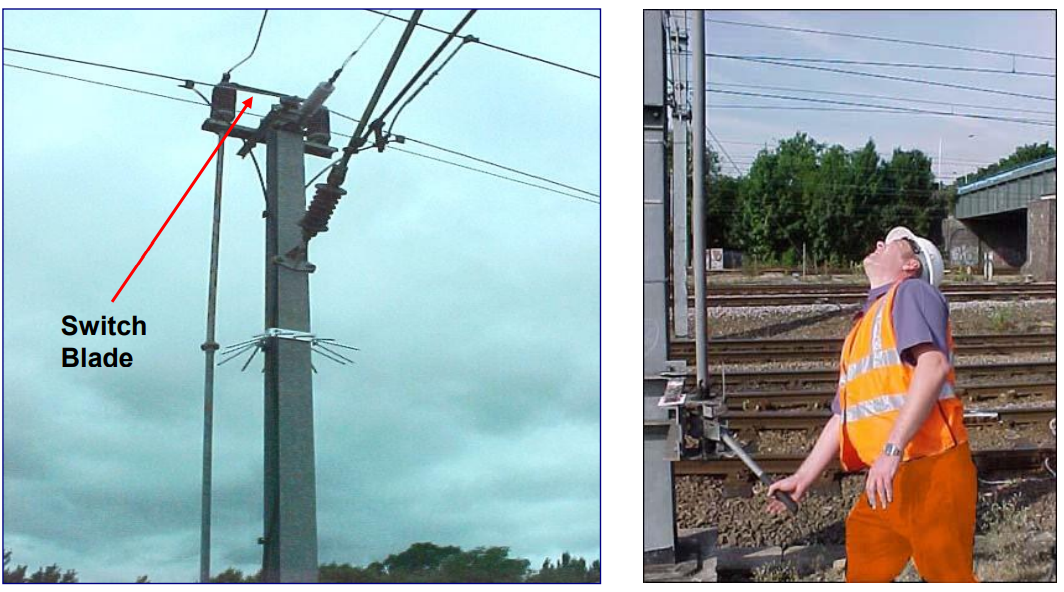
\includegraphics[width = 0.8\textwidth]{img/figure145.png}
    \caption{Isolator / switches.}
\end{figure}
The electrical sections can be split into sub-sections by means of manually operated or motorised switches.
\begin{figure}[H]
    \centering
    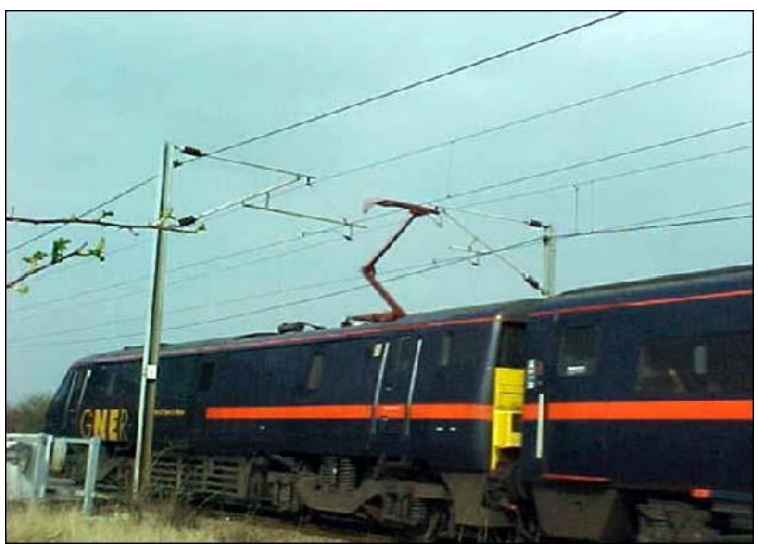
\includegraphics[width = 0.8\textwidth]{img/figure146.png}
    \caption{Pantograph.}
\end{figure}
The current is collected from the OLE via a pantograph and passes through the train's traction equipment before passing through its axles and wheels to the traction return rail. 
\section{MAGLEV Systems}
\begin{figure}[H]
    \centering
    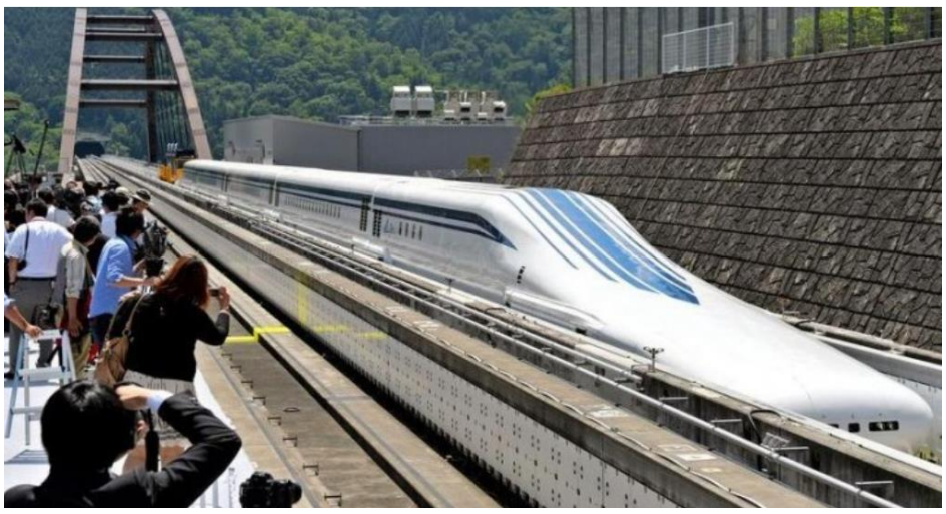
\includegraphics[width = 0.7\textwidth]{img/figure147.png}
    \caption{MAGLEV Train from Japan.}
\end{figure}
Japan Railways' latest mag-lev bullet train broke its own record as the fastest train in the world \SI{603}{\kilo\meter\per\hour}. Carries just over 900 passengers per trip as it levitates above the track using electromagnets to create a nearly frictionless ride. 
\section{Question 3 - What are the main advantages of the 25 kV overhead system over the 750 V DC third rail system?}
The higher level of power that is attainable from the high voltage system and ability to transform it to appropriate voltage levels for different speeds i.e. by using a tap transformer. 
\section{Question 4 - Consider the merits and demerits of electric traction systems}
\subsection{Merits of electric traction}
\begin{itemize}
    \item High starting torque
    \item Less maintenance cost
    \item Cheapest method of traction
    \item Rapid acceleration and braking
    \item Less vibration
    \item Free from smoke and flue gases hence used for underground and tubular railway
\end{itemize}
\subsection{Demerits of electric traction}
\begin{itemize}
    \item High capital cost
    \item Problem of supply failure
    \item Additional equipment is required for achieving electric braking and control - regenerative energy is possible
    \item The electrically operated vehicles have to move on guided track only - suburban routes
\end{itemize}